\documentclass[11pt]{article}

\usepackage{amssymb,amsmath,amsfonts,amsthm}
\usepackage{latexsym}
\usepackage{graphics}
\usepackage{indentfirst}
\usepackage{lmodern}
\usepackage{hyperref}
\usepackage{mathrsfs}
\usepackage{array}
\usepackage{mathtools}
\usepackage{graphicx}
\usepackage{setspace}
\usepackage{enumerate}
\usepackage{tikz}
\usepackage{url,color}
\usepackage{xcolor}
\usepackage{chngcntr}
\usepackage{multicol}
\usepackage{comment}
\usepackage{float}
\usepackage{algpseudocode}
\usepackage{subcaption}
\usepackage[ruled]{algorithm2e}
\usepackage{booktabs}
\usepackage{caption}
\usepackage[letterpaper,margin=2cm,top=2.5cm,bottom=2.5cm]{geometry}

\AtBeginEnvironment{algorithm}{\setstretch{1.2}}

\hypersetup{colorlinks=true,citecolor=blue,linkcolor=blue,urlcolor=blue}

%%%%%%%%%%%%%%%%%%%%%%%%%%%%%%%%%%%%%%%%%%%%%%%%%%%%%%%%%%
%% Theorem environments
%%%%%%%%%%%%%%%%%%%%%%%%%%%%%%%%%%%%%%%%%%%%%%%%%%%%%%%%%%
\newtheorem{theorem}{Theorem}[section]
\newtheorem{lemma}{Lemma}[section]
\newtheorem{proposition}{Proposition}[section]
\newtheorem{corollary}{Corollary}[section]
\newtheorem{claim}{Claim}[section]
\newtheorem{conjecture}{Conjecture}[section]
\newtheorem{hypothesis}{Hypothesis}[section]
\newtheorem{assumption}{Assumption}[section]
\newtheorem{remark}{Remark}[section]
\newtheorem{example}{Example}[section]
\newtheorem{problem}{Problem}[section]
\newtheorem{definition}{Definition}[section]
\newtheorem{question}{Question}[section]
\newtheorem{condition}{Condition}[section]

%%%%%%%%%%%%%%%%%%%%%%%%%%%%%%%%%%%%%%%%%%%%%%%%%%%%%%%%%%
%% Math shorthands
%%%%%%%%%%%%%%%%%%%%%%%%%%%%%%%%%%%%%%%%%%%%%%%%%%%%%%%%%%
\newcommand{\N}{\mathbb{N}}
\newcommand{\Z}{\mathbb{Z}}
\newcommand{\E}{\mathbb{E}}
\newcommand{\Q}{\mathbb{Q}}
\newcommand{\R}{\mathbb{R}}
\newcommand{\C}{\mathbb{C}}
\newcommand{\norm}[1]{\left\lVert#1\right\rVert}

\allowdisplaybreaks

%%%%%%%%%%%%%%%%%%%%%%%%%%%%%%%%%%%%%%%%%%%%%%%%%%%%%%%%%%
%% Title, authors, abstract
%%%%%%%%%%%%%%%%%%%%%%%%%%%%%%%%%%%%%%%%%%%%%%%%%%%%%%%%%%

\title{Anchored Integer Refinement of Redistricting Plans:\\
       A Kernel-Aware Matheuristic and Its Benchmarks}

\author{Alaittin K\i rt\i \c{s}o\u{g}lu \\
        \small Department of Applied Mathematics, Illinois Institute of Technology \\
        \small Chicago, IL 60616 \\
        \small \texttt{kirtisoglu@hawk.iit.edu}}

\date{\today}

\begin{document}
\maketitle

\begin{abstract}
We study the integer form of a diffusion energy for redistricting, a
kernel-weighted Laplacian cut term plus a fidelity term that anchors
each move to the current plan, solved as a convex mixed-integer
program on a merged pair of districts inside a tempered recombination
chain. The result is a matheuristic ensemble generator, not a
sampler, and we evaluate it as one. On Iowa it reduces mean cut edges
by 20 percent over tempered ReCom across ten seeds, but simulated
annealing over ReCom proposals reaches the same best plans at a
fraction of the cost, so its value is anchored, kernel-aware
refinement near a reference plan. We quantify that niche in a
least-change experiment from Iowa's enacted map, where it ties the
best annealer at a ten-county budget and is the only deterministic
method, and in a multi-kernel showcase where perimeter and density
kernels produce measurably different plans. A continuous relaxation
with Cheeger-sweep rounding and a spectral mixture are reported as
null results. The theory of the proposal, its exact correction, and
the resulting sampler appear in a companion paper.
\end{abstract}

%% DRAFT SKELETON assembled 2026-10-13 from the blocks split out of the
%% companion paper. Sections 2 and 3 are copied background; the intro,
%% discussion and conclusion are stubs to be written. References to
%% the companion paper appear as "Paper~I".

%════════════════════════════════════════════════════════════════════════════════
\section{Introduction}\label{sec:intro}
%════════════════════════════════════════════════════════════════════════════════

%% TODO: write. The pitch is honest matheuristic evaluation: an anchored,
%% kernel-aware MIQP refinement inside a tempered recombination chain,
%% benchmarked against the classical optimizers a referee should demand
%% (annealing, hill climbing, restarts), against Dobbs et al.'s exact
%% transfer-distance programs in the least-change setting, and positioned
%% in the Brous--Shmoys / Gurnee--Shmoys / Swamy et al. lineage.

%════════════════════════════════════════════════════════════════════════════════
\section{Background: plans and ReCom}\label{sec:background}
%════════════════════════════════════════════════════════════════════════════════

\subsection{Dual graph and \texorpdfstring{$k$}{k}-district plans}\label{sec:background-graph}

Let $G = (V, E)$ be the dual graph of a state, with vertices
representing geographic units (precincts, census blocks, counties) and
edges encoding shared boundaries. Each vertex $v$ carries a population
$p_v \ge 0$ and may carry additional attributes (demographic vectors,
shapefile geometry). A \emph{$k$-district plan} is a partition
$P = \{V_1, \ldots, V_k\}$ of $V$ such that each induced subgraph
$G[V_i]$ is connected (\emph{contiguity}) and the populations satisfy
\begin{equation}\label{eq:pop-balance}
  (1 - \varepsilon)\bar p \;\le\; p(V_i) \;\le\; (1 + \varepsilon)\bar p,
  \qquad \bar p := \frac{p(V)}{k},
\end{equation}
for a tolerance $\varepsilon \in [0, 1)$. We write $\mathcal{P}_k(G; \varepsilon)$
for the set of valid plans. The \emph{cut edges} of a plan are
\[
  \partial P \;=\; \{(u,v) \in E : P(u) \ne P(v)\},
\]
and we call $|\partial P|$ the \emph{cut-edge count} of $P$. This
quantity is the discrete analog of the perimeter of the district
boundaries and serves as our primary compactness
metric~\cite{duchin2018discrete}.

\begin{figure}[htbp]
  \centering
  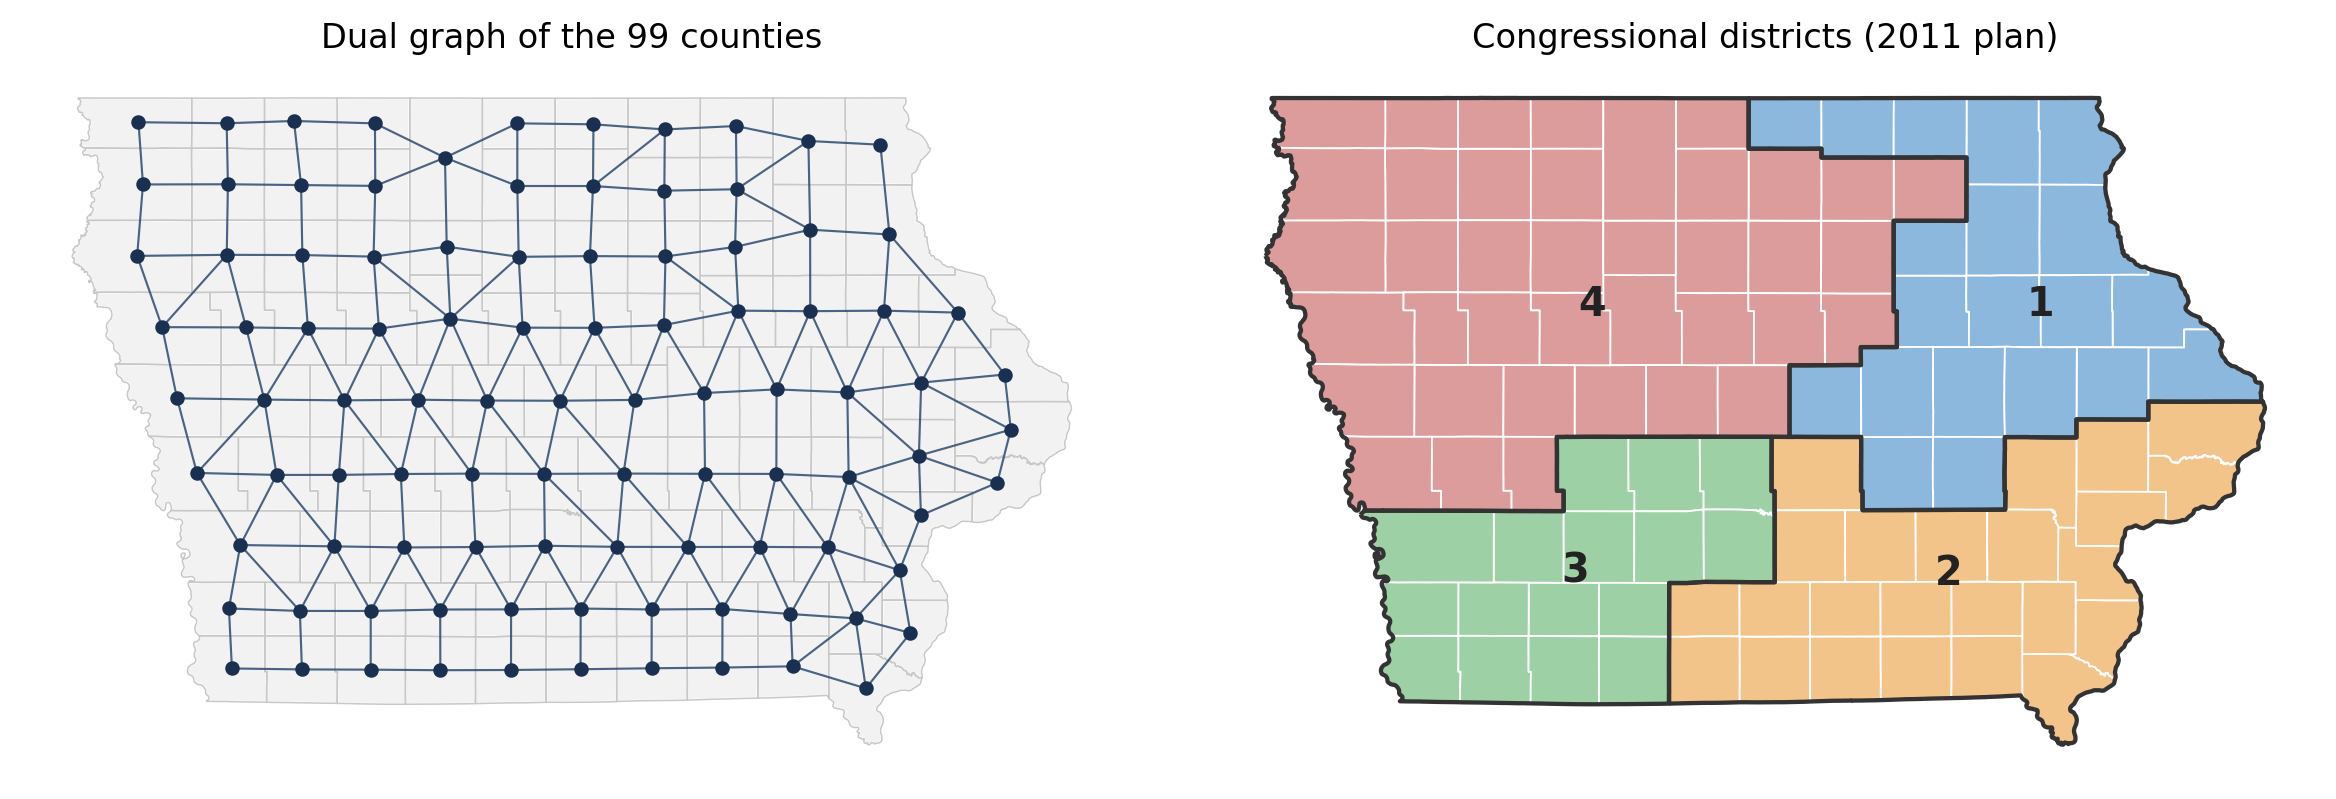
\includegraphics[width=0.5\textwidth]{fig/redistricting.png}
  \caption{The dual graph of Iowa's 99 counties (left) and the four
    congressional districts enacted after the 2010 census (right).
    Nodes sit at county centroids; two counties are joined by an edge
    when they share a boundary segment.}
  \label{fig:iowa-dual}
\end{figure}

\subsection{Recombination (ReCom)}\label{sec:background-recom}

Recombination~\cite{deford2021recombination} is a Markov chain on
$\mathcal{P}_k(G; \varepsilon)$ whose single step is given in Algorithm~\ref{alg:recom}.

\begin{algorithm}[H]
\caption{Vanilla ReCom step (Chain V)}\label{alg:recom}
\KwIn{Current plan $P$, dual graph $G$, balance tolerance $\varepsilon$.}
\KwOut{Next plan $P'$.}
Select two adjacent districts $V_i, V_j$ uniformly at random from boundary pairs;\\
Form the induced subgraph $H = G[V_i \cup V_j]$;\\
\Repeat{a cut $e^*$ exists yielding two $\varepsilon$-balanced components}{
  Sample a uniform random spanning tree $T$ of $H$ via Wilson's algorithm~\cite{wilson1996generating};\\
  Search edges of $T$ for a cut $e^*$ whose removal produces two $\varepsilon$-balanced components.
}
Define $V_i', V_j'$ as the two components of $T \setminus \{e^*\}$;\\
$P' \gets P$ with $V_i, V_j$ replaced by $V_i', V_j'$;\\
\Return $P'$.
\end{algorithm}

\noindent The tree-based proposal flips many precincts simultaneously
between $V_i$ and $V_j$ while preserving contiguity automatically (any
edge removal from a tree produces two connected components). This is
the key advantage over single-precinct flip chains, which traverse the
state space too slowly to be practically useful.

\textbf{Chains compared.} We compare six chains, three of them from
this work (Table~\ref{tab:five-chains}).

\begin{table}[htbp]
\centering
\small
\begin{tabular}{llll}
\toprule
Chain & Method & Mechanism & Stationarity claim \\
\midrule
V & Vanilla ReCom~\cite{deford2021recombination} & spanning-tree split, always accept & unknown target \\
A & Tempered ReCom & ReCom + MH on cuts (symmetric-$q$) & approximate \\
B & ReCom + QP-diffusion mix (this work) & continuous QP, Cheeger sweep, repair & none (heuristic) \\
C & Tempered ReCom + IQP local (this work) & MIQP refinement, orphan-flip repair & none (matheuristic) \\
D & ReCom + spectral mix (after~\cite{davies2025spectral}) & Fiedler + balanced sweep, no $\beta$, no repair & none (heuristic) \\
E & QP-MH (this work, Paper~I, \S4.6) & QP + Bernoulli rounding + exact MH & \textbf{exact} \\
\bottomrule
\end{tabular}
\caption{The six chains compared in this paper. The last column is the
  chain's relationship to the tempered target
  $\pi(P) \propto \exp(-\lambda|\partial P|)$. Only Chain E carries an
  exact Metropolis--Hastings correction; Chains B--D are heuristics
  whose output distributions we characterize empirically, and Chain A
  relies on the symmetric-$q$ approximation
  (Paper~I, \S4.6).}
\label{tab:five-chains}
\end{table}

Tempered ReCom uses a Metropolis--Hastings filter targeting
$\pi(P) \propto \exp(-\lambda |\partial P|)$ with the symmetric-$q$
approximation (treating the forward and reverse proposal probabilities
as equal); see Appendix~\ref{app:hyperparams} for the locked-in
$\lambda = 0.10$. Our Chain D departs from published SpecReCom in one
deliberate way. Instead of the sign split of the Fiedler vector (which
ignores population balance), it runs our balance-constrained Cheeger
sweep over the Fiedler order, closer in spirit to BalSpecReCom, so that all chains produce valid plans and the comparison isolates the
role of the fidelity term. All chains also enforce the global
two-sided balance window of Equation~\eqref{eq:balance-window} on
every move; we note (\S\ref{sec:exp-balance}) that the raw GerryChain
\texttt{recom} proposal alone does not.

\paragraph{The proposal we replace.}\label{sec:background-weakness}
The tree-and-cut step is kernel-blind (Paper~I, \S1.1),
and the cut edge is chosen only after the tree is drawn, so the
proposal cannot anticipate the shape of the split. The diffusion
proposal of \S\ref{sec:model} replaces that step with a single convex
optimization of a kernel-weighted Laplacian energy plus a
locality-preserving fidelity term. The energy
$x^\top L\, x = \sum_{(u,v) \in E} w_{uv} (x_u - x_v)^2$ equals the
weighted cut count for binary $x$, so minimizing it directly
minimizes the discrete perimeter in the chosen kernel.

%════════════════════════════════════════════════════════════════════════════════
\section{The energy and its kernels}\label{sec:model}
%════════════════════════════════════════════════════════════════════════════════

\subsection{Locality kernels}\label{sec:kernels}

Choosing the edge weights $w_{ij}$ is the most important modeling
decision. The kernel determines what \emph{smoothness} means and
therefore controls how district boundaries move under the relaxation.
We restrict all weights to geographic neighbors,
\begin{equation}\label{eq:kernel-local}
  w_{ij} = 0 \quad \text{if } (v_i, v_j) \notin E,
\end{equation}
ensuring that diffusion operates only through geographic adjacency and
preventing long-range interactions that could produce disconnected
districts.

\paragraph{Uniform kernel ($k_{\mathrm{unif}}$).} $w_{ij} = 1$ for
every edge. The Laplacian $L$ is the combinatorial graph Laplacian;
$x^\top L x$ is exactly the cut edge count. In the $\beta \to 0^+$
limit the proposal approaches a balanced Fiedler-style split
(\S\ref{sec:iqp-subsumption}).

\paragraph{Perimeter kernel ($k_{\mathrm{perim}}$).} $w_{ij} = |\partial v_i \cap \partial v_j|$
(shared-boundary length). The Laplacian quadratic form $x^\top L x$
is then the \emph{geographic perimeter} of the partition, weighted by
boundary segment length. This kernel discourages fragmented districts
and favors boundaries that cut along short segments.

\paragraph{Density kernel ($k_{\mathrm{dens}}$).} Let $\rho_v$ denote
the population density at vertex $v$ (population per unit area). A
Gaussian density kernel
\[
  w_{ij} \;=\; |\partial v_i \cap \partial v_j| \cdot
  \exp\!\Bigl( -\frac{(\rho_i - \rho_j)^2}{\sigma^2} \Bigr)
\]
encourages cuts along sharp density gradients (urban--rural
boundaries) while preserving the topological role of shared boundary
length.

\paragraph{Demographic kernel ($k_{\mathrm{demog}}$).} Let
$d_v \in \R^m$ be a vector of demographic attributes. A Gaussian
similarity kernel $w_{ij} = \exp(-\|d_i - d_j\|^2 / \sigma^2)$
encourages communities of interest. We define this kernel for
completeness but do not use it in our experiments, and a caution
stronger than ``use as a soft regularizer'' is warranted. If the
attribute vector encodes race, a proposal that systematically shapes
district boundaries around racial similarity risks making race the
predominant districting criterion, which triggers strict scrutiny
under the \emph{Shaw v.\ Reno} line of racial-gerrymandering cases.
Any practical use of demographic kernels should be reviewed against
that doctrine, should document the kernel's weight relative to
race-neutral criteria, and is more defensible for attributes that are
legitimate districting factors in the jurisdiction (e.g., municipal
membership, communities of interest as defined by state law).

\paragraph{Composite kernels.} Linear combinations $w_{ij} = \sum_k a_k w_{ij}^{(k)}$
with $a_k \ge 0$ remain valid, since they preserve nonnegativity and locality.

\subsection{The convex QP}\label{sec:qp-model}

Let $H = G[V_i \cup V_j]$ be the merged subgraph of two adjacent
districts. Let $L_H$ be the kernel-weighted Laplacian of $H$, let
$x_0 \in \{0,1\}^{|V_H|}$ encode the current bipartition (1 for
vertices in $V_i$, 0 for vertices in $V_j$), and let $p$ be the
population vector restricted to $H$. Fix weights $\alpha, \beta > 0$
and balance tolerance $\varepsilon \in (0, 1)$. Crucially, the balance
constraint is anchored to the \emph{global} per-district ideal
$\bar p = p(V)/k$ from Equation~\eqref{eq:pop-balance}, not to
$p(V_H)/2$. Both sides of the split must individually satisfy the
plan-validity bound, which yields the two-sided window
\begin{equation}\label{eq:balance-window}
  \ell \;=\; \max\bigl((1-\varepsilon)\bar p,\; p(V_H) - (1+\varepsilon)\bar p\bigr),
  \qquad
  u \;=\; \min\bigl((1+\varepsilon)\bar p,\; p(V_H) - (1-\varepsilon)\bar p\bigr).
\end{equation}
Anchoring to $p(V_H)/2$ instead (a tempting simplification, and one
present in an earlier version of our own implementation) only bounds
the local split. Because $p(V_H)$ itself drifts as the chain moves
population between pairs, district populations can ratchet outside the
global tolerance by a factor of up to $(1+\varepsilon)$ per move on
heterogeneous graphs. Our experiments audit the global bound at every
step (\S\ref{sec:experiments}).

\begin{definition}[Continuous QP-diffusion]\label{def:qp}
The continuous QP-diffusion bipartition of $H$ is
\begin{align}
  x^\star \;=\; \arg\min_{x \in [0,1]^{|V_H|}} \;\;
    & \alpha\, x^\top L_H\, x \;+\; \beta\, \|x - x_0\|_2^2 \label{eq:qp-obj} \\
  \text{subject to} \;\;
    & \ell \;\le\; p^\top x \;\le\; u,
    \label{eq:qp-balance}
\end{align}
with $\ell, u$ as in Equation~\eqref{eq:balance-window}.
\end{definition}

The first term in~\eqref{eq:qp-obj} is the kernel-weighted Laplacian
smoothness energy. For binary $x$ it equals the weighted cut count
$\sum_{(u,v) \in E(H)} w_{uv}\,\mathbf{1}[x_u \ne x_v]$, and the
continuous relaxation $x \in [0,1]^{|V_H|}$ extends this to a smooth
objective on the unit cube. The second term is the \emph{fidelity term},
which penalizes deviation from the current bipartition and ensures
that each proposed move is local. The balance constraint enforces
$\varepsilon$-balance on the proposed split.

\begin{proposition}[Convexity and well-posedness]\label{prop:convex}
The objective in~\eqref{eq:qp-obj} is strictly convex on
$[0,1]^{|V_H|}$ (since $\beta > 0$ and $L_H$ is positive semidefinite).
The feasible region defined by~\eqref{eq:qp-balance} is a nonempty
polytope whenever the current plan is valid (it then contains $x_0$).
Hence the QP admits a unique minimizer $x^\star$, computable in
polynomial time by any convex QP solver.
\end{proposition}

\paragraph{Spectral interpretation.} Projecting the interior optimality
condition $(\alpha L_H + \beta I) x^\star = \beta x_0$ onto the
eigenbasis $\{\phi_k\}$ of $L_H$ with eigenvalues
$0 = \lambda_1 \le \lambda_2 \le \cdots \le \lambda_n$ yields the
closed-form frequency response
\begin{equation}\label{eq:freq-response}
  \hat x^\star_k \;=\; \frac{\beta}{\alpha \lambda_k + \beta}\,
  \hat x_{0,k},
  \qquad \hat y_k := \phi_k^\top y.
\end{equation}
The QP therefore acts as a low-pass spectral filter on the prior $x_0$,
with cutoff controlled by the ratio $\alpha / \beta$. Equivalently, with
$\tau := \alpha / \beta$, the optimum satisfies
$(x^\star - x_0)/\tau = -L_H x^\star$, the implicit Euler
discretization of the graph heat equation $\dot x = -L_H x$. Inspecting
the leading eigenvectors $\phi_2, \phi_3, \ldots$ provides a sanity
check on kernel choice. If they look like noise rather than coherent
geographic regions, the chosen kernel is probably not informative.

\subsection{Cheeger-sweep rounding and orphan-flip repair}\label{sec:rounding}

The continuous optimum $x^\star \in [0,1]^{|V_H|}$ must be rounded to a
binary bipartition. We use a \emph{Cheeger sweep}~\cite{chung1997spectral}. Sort the entries of $x^\star$ in descending order, and for each
threshold $k = 1, \ldots, |V_H| - 1$ form the candidate set $S_k$ of the
top-$k$ vertices. Among candidates that satisfy $\varepsilon$-balance,
return the one minimizing the cut count
$|\partial(S_k, V_H \setminus S_k)|$. Candidates with disconnected sides
are passed through the orphan-flip repair below before evaluation.

\begin{algorithm}[H]
\caption{Cheeger-sweep rounding with orphan-flip repair}\label{alg:cheeger-sweep}
\KwIn{Continuous optimum $x^\star \in [0,1]^{|V_H|}$, population
  vector $p$, target $\bar p$, tolerance $\varepsilon$, merged subgraph $H$.}
\KwOut{Binary bipartition $S \subset V_H$ or \texttt{FAIL}.}
Sort $V_H$ by $x^\star$ descending; call the order $v_{(1)}, \ldots, v_{(|V_H|)}$;\\
$\mathcal{C} \gets \emptyset$ \tcp*{candidates}
\For{$k = 1$ \KwTo $|V_H| - 1$}{
  $S_k \gets \{v_{(1)}, \ldots, v_{(k)}\}$;\\
  \uIf{$p(S_k) \in [(1-\varepsilon)\bar p, (1+\varepsilon)\bar p]$ and both sides connected}{
    Add $S_k$ to $\mathcal{C}$ with cut $|\partial(S_k, V_H \setminus S_k)|$;
  }\ElseIf{$p(S_k)$ in balance and sides have $> 1$ components}{
    $S_k' \gets$ orphan-flip repair of $S_k$ (Algorithm~\ref{alg:orphan-flip});\\
    \If{$S_k'$ satisfies balance and connectivity}{
      Add $S_k'$ to $\mathcal{C}$;
    }
  }
}
\lIf{$\mathcal{C} = \emptyset$}{\Return \texttt{FAIL}}
\Return $\arg\min_{S \in \mathcal{C}} |\partial(S, V_H \setminus S)|$.
\end{algorithm}

The sweep can return a candidate $S_k$ whose induced subgraph $G[S_k]$
or $G[V_H \setminus S_k]$ is disconnected. A single boundary vertex
on the wrong side of the threshold is enough. Discarding such
candidates outright would inflate the rejection rate; instead we repair
them. The \emph{orphan-flip} routine identifies the disconnected
components of each side, keeps the largest component, and flips every
smaller (\emph{orphan}) component to the opposite side. Population
balance is then re-verified; if the repair preserves both balance and
connectivity, the repaired candidate enters the Cheeger sweep's
candidate pool. Algorithm~\ref{alg:orphan-flip} formalizes this procedure.

\begin{algorithm}[H]
\caption{Orphan-flip repair}\label{alg:orphan-flip}
\KwIn{Candidate bipartition $(S, V_H \setminus S)$.}
\KwOut{Repaired bipartition or \texttt{FAIL}.}
Identify connected components of $G[S]$ and $G[V_H \setminus S]$;\\
\For{each side}{
  Keep the largest connected component;\\
  Flip every smaller component to the opposite side;
}
Verify both final sides are connected and $\varepsilon$-balanced;\\
\lIf{verification fails}{\Return \texttt{FAIL}}
\Return repaired $(S', V_H \setminus S')$.
\end{algorithm}

\textbf{Why repair matters.} On heterogeneous-population graphs such
as Iowa, the unrepaired Cheeger sweep produces near-feasible
candidates whose few orphan vertices (often singletons at the
boundary) can be reassigned without affecting the cut count.
Without repair, post-rounding rejection rates on Iowa run at 5--15\%;
with repair, $<3\%$. SpecReCom~\cite{davies2025spectral} does not use
repair (and we keep it out of our faithful Chain D
implementation); without the $\beta$ fidelity term, repair tends to
accept lower-quality cuts.

\paragraph{On sweep guarantees.} We do not claim the Cheeger
bound~\cite{chung1997spectral} for the rounded solution. The sweep is
applied to the constrained proximal optimum of
Definition~\ref{def:qp}, not to the Fiedler vector, and the balance
restriction on admissible thresholds voids the standard argument, so
the sweep is a rounding heuristic whose output we measure. It also
selects the candidate minimizing the \emph{unweighted} cut even when
the energy uses a non-uniform kernel, a configuration choice we flag
in \S\ref{sec:exp-multikernel}.

\subsection{Hybrid composition with ReCom (Chain B)}\label{sec:hybrid-mh}

Chain B's single step is a random mixture. With probability
$p_R = 0.5$, take a Vanilla ReCom step (Algorithm~\ref{alg:recom});
otherwise take a QP-diffusion step (Definition~\ref{def:qp} and
Algorithm~\ref{alg:cheeger-sweep}). We state plainly what Chain B is
and is not. \emph{Neither branch carries a Metropolis correction}, the ReCom branch always accepts (as in Vanilla ReCom), and the
QP-diffusion branch applies the rounded, repaired split
unconditionally. Chain B therefore has no stationarity claim beyond
ergodicity; it is an exploratory heuristic whose empirical output
distribution we characterize against enumerated ground truth in
Paper~I, \S5.1. The exactly corrected sampler built from the same
proposal is Chain E (Paper~I, \S4.6).

\begin{proposition}[Ergodicity of the hybrid]\label{prop:ergodic}
If ReCom is ergodic on $\mathcal{P}_k(G; \varepsilon)$ (which holds
under standard assumptions; see~\cite{deford2021recombination,
cannon2024irreducibility}), then the mixture of ReCom and
the QP-diffusion step with any $p_R \in (0, 1)$ is also ergodic.
\end{proposition}

\begin{proof}
Write the mixture kernel as $K = p_R K_{\mathrm{R}} +
(1 - p_R) K_{\mathrm{Q}}$. If $K_{\mathrm{R}}^{T}(P, P') > 0$ for
some $T$, then $K^{T}(P, P') \ge p_R^{T}\, K_{\mathrm{R}}^{T}(P, P')
> 0$, so irreducibility of ReCom implies irreducibility of the
mixture. For aperiodicity, the ReCom branch already holds in place
with positive probability. The current split of any selected pair is
a balanced bipartition of the connected merged subgraph $H$, and it
is produced whenever the sampled spanning tree consists of a spanning
tree of each side joined by one crossing edge, an event of positive
probability under the uniform tree measure. Hence
$K_{\mathrm{R}}(P, P) > 0$, so $K(P, P) > 0$ for every $P$ and the
chain is aperiodic.
\end{proof}

\subsection{The integer QP-diffusion (Chain C)}\label{sec:iqp}

The integer counterpart of Definition~\ref{def:qp} replaces
$x \in [0,1]^{|V_H|}$ with $x \in \{0, 1\}^{|V_H|}$ and solves the
resulting mixed-integer convex quadratic program (MIQP) directly.

\paragraph{Definition and solver.}\label{sec:iqp-def}

\begin{definition}[Integer QP-diffusion]\label{def:iqp}
The IQP local refinement of $H$ is
\begin{align}
  x^\star \;=\; \arg\min_{x \in \{0,1\}^{|V_H|}} \;\;
    & \alpha\, x^\top L_H\, x \;+\; \beta\, \|x - x_0\|_2^2 \label{eq:iqp-obj} \\
  \text{subject to} \;\;
    & \ell \;\le\; p^\top x \;\le\; u,
\end{align}
with the same global-ideal balance window $(\ell, u)$ of
Equation~\eqref{eq:balance-window} as the continuous case.
\end{definition}

The objective is convex quadratic and the variable is binary.
Gurobi's MIQP solver handles this directly via branch-and-bound; in
practice, a 5-second time limit per solve is rarely hit on Iowa-sized
merged pairs ($\sim 30$--$60$ precincts).

\paragraph{Subsumption of cut-min; relation to SpecReCom.}\label{sec:iqp-subsumption}

\begin{proposition}[Special cases]\label{prop:iqp-special-cases}
Setting $\alpha = 1$, $\beta = 0$, $w_{ij} \equiv 1$ in
Definition~\ref{def:iqp} gives the classical minimum-cut integer
program subject to the balance window. Hence Chain C subsumes
the discrete cut-minimization MIP as a special case.
\end{proposition}

We are careful \emph{not} to claim the analogous statement for the
continuous case. At $\beta = 0$ the relaxation of
Definition~\ref{def:qp} is degenerate. Any feasible constant vector
$c\mathbf{1}$ attains energy zero, so the minimizer carries no cut
information and the sweep is undefined. SpecReCom's Fiedler direction
arises from the Rayleigh quotient \emph{restricted to}
$x \perp \mathbf{1}$, a constraint our proximal program does not
impose; it is the fidelity term ($\beta > 0$) that breaks the constant
degeneracy here, with $x_0$ playing the symmetry-breaking role that
orthogonality plays in spectral partitioning. The precise relationship
is that as $\beta \to 0^+$ with $x_0$ non-constant, the minimizer's
projection off $\mathbf{1}$ aligns with the low-frequency eigenspace
of $L_H$ (Equation~\eqref{eq:freq-response} with
$\beta/(\alpha\lambda_k + \beta) \to 0$ fastest at high frequencies),
so Chain B approaches a Fiedler-like split \emph{in direction} while
retaining balance feasibility. This gives a BalSpecReCom-style variant rather
than SpecReCom itself. Chain D implements that variant directly.

\paragraph{Locality via the fidelity term.}\label{sec:iqp-locality}

For $\beta = 0$, the IQP optimum is a minimum cut of $H$ subject only
to population balance and may differ arbitrarily from $x_0$. For
$\beta > 0$ the optimum is biased toward $x_0$, since every flip
incurs a $\beta$ penalty, so the proposed split stays near the current
one, is mostly contiguous already because $x_0$ is, and needs only a
few boundary units repaired; the rejection figures of
\S\ref{sec:rounding} are the measured consequence.

\paragraph{One step of Chain C.}\label{sec:chain-c-step}
A single step of Chain C wraps an outer Tempered ReCom move
(Algorithm~\ref{alg:recom} plus the Metropolis--Hastings filter of
\S\ref{sec:hybrid-mh}) around $n_{\mathrm{iqp}}$ deterministic
IQP local-refinement passes. Each inner pass picks an adjacent district
pair, solves the IQP on the merged subgraph, and applies orphan-flip
repair; if the repair fails the inner pass leaves the plan unchanged.
The full step is given as Algorithm~\ref{alg:chain-c}.

\begin{algorithm}[H]
\caption{One step of Chain C}\label{alg:chain-c}
\KwIn{Current plan $P$, parameters $\alpha, \beta, n_{\mathrm{iqp}}, \lambda, \varepsilon$.}
\KwOut{Next plan $P'$.}
$P_0 \gets $ Tempered ReCom step (Chain A) applied to $P$\;
$P_{\mathrm{curr}} \gets P_0$\;
\For{$t = 1$ \KwTo $n_{\mathrm{iqp}}$}{
  Select adjacent district pair $(V_i, V_j)$ uniformly from boundary pairs of $P_{\mathrm{curr}}$\;
  Form $H = G[V_i \cup V_j]$, build kernel-weighted $L_H$\;
  Solve IQP (Definition~\ref{def:iqp}) for $x^\star$\;
  Apply orphan-flip repair (Algorithm~\ref{alg:orphan-flip})\;
  \uIf{repaired bipartition feasible and connected}{
    Update $V_i, V_j$ in $P_{\mathrm{curr}}$ to the new bipartition\;
  }\Else{
    $P_{\mathrm{curr}}$ unchanged\;
  }
}
\Return $P' \gets P_{\mathrm{curr}}$.
\end{algorithm}

\paragraph{What Chain C is, and is not.}\label{sec:chain-c-honest}
The IQP loop is \emph{deterministic} given the random pair choices. There is no Metropolis acceptance inside the loop, and the outer
acceptance applies only to the Tempered ReCom move. We are explicit
about the consequence. \textbf{Chain C is not a sampler for the
tempered target} $\pi(P) \propto \exp(-\lambda|\partial P|)$, and no
completion of the construction can make it one. A deterministic map
$T$ composed after a $\pi$-invariant kernel preserves $\pi$ only if
$T$ is itself $\pi$-preserving (essentially a $\pi$-preserving
involution~\cite{tierney1998note}), whereas the IQP refinement is a
many-to-one, cut-decreasing contraction onto local minima, the
opposite of an involution. Nor can the refinement be folded into the
proposal and Metropolized, since the reverse move would require the
argmin at $P'$ to output the strictly worse plan $P$, an event of
probability zero. The distributional signature of this bias is visible
in our own ground-truth data (Paper~I, \S5.1), where Chain C's cut
marginal is shifted and sharply concentrated relative to Chain A's,
despite the identical outer kernel.

We therefore present Chain C as what it is, a \emph{matheuristic
ensemble generator} in the lineage of ReCom-based
optimization~\cite{cannon2023voting,brous2025recom}, an iterated
local search whose stochastic component (the tempered outer move)
maintains diversity while the embedded MIQP drives compactness. This
is a legitimate and, as \S\ref{sec:experiments} shows, empirically
powerful tool for producing high-quality compact plans and for
seeding or stress-testing ensembles. What it does not provide is a
defensible null distribution for outlier analysis; for that use case
the field's requirements are exactly the known-target
property~\cite{cannon2022spanning,mccartan2023sequential} that
Chain E (Paper~I, \S4.6) preserves and Chain C deliberately trades
away for optimization power.

\paragraph{Trade-off: continuous vs.\ integer.}\label{sec:iqp-pareto}
The continuous relaxation is roughly $45\times$ cheaper per step in
wall-clock (a linear solve in the common case, by
Paper~I, Lemma~4.1), but on Iowa only the exact integer
solve moves the compactness needle; the contrast is developed in
\S\ref{sec:exp-compactness}.

%════════════════════════════════════════════════════════════════════════════════
\section{Experiments}\label{sec:experiments}
%════════════════════════════════════════════════════════════════════════════════

We evaluate the six chains of Table~\ref{tab:five-chains} on three
datasets, namely the $5 \times 5$ grid (full enumeration, ground-truth
target), the Iowa county dual graph (real geography, 99 counties,
$k = 4$, $\varepsilon = 0.05$), and the North Carolina precinct dual
graph ($2\,692$ precincts, $k = 4$, $\varepsilon = 0.05$). All hyperparameters are
locked in Appendix~\ref{app:hyperparams}; raw cut traces, per-step
balance audits, and configuration stamps are released in the project
repository.

\paragraph{Statistical protocol.} Chains are autocorrelated, so we do
not report i.i.d.\ test statistics on raw traces. For every
comparison we report the mean difference, Cohen's $d$ on the pooled
post-burn-in standard deviation, and a $z$-test whose standard errors
use effective sample sizes (ESS) from Geyer's initial-positive-sequence
estimator of the integrated autocorrelation time. ESS values are
reported alongside and are small, typically tens per 400 retained
Iowa steps (as low as 3 for Chain E). On the $5 \times 5$ grid Chain
C's trace is nearly constant and the estimator is unstable there, so
we draw no single-run inference from it and let the ten-seed
comparisons carry that claim. All ESS values are computed from cut
traces and are appropriate for inference about cut means only;
distributional tests use batch means (Paper~I, \S5.2).
Each chain runs on its own seeded RNG stream. The tables below report
a single seed (42) with full diagnostics; every headline comparison
was replicated across ten seeds (42 through 51) under one solver
configuration. On Iowa, Chain C's gain is $-8.0 \pm 0.4$ cuts versus
Chain A ($-20.3\%$), negative on all ten seeds (paired
$p = 6.4 \times 10^{-13}$), with C's mean cut count at
$31.4 \pm 0.3$. Chain B's effect resolves to $-0.9 \pm 0.9$ cuts (population
standard deviation, as in every table)
($-2.3\%$), negative on nine of ten seeds and nominally significant
($p = 0.015$) but an order of magnitude below C's, so single runs
cannot distinguish it from zero. Chain D is indistinguishable from A
($+0.4$ cuts, $p = 0.10$). On the $5 \times 5$ fiber, C's between-seed
spread is essentially nil ($16.03 \pm 0.02$ mean cuts) and its
$-4.0\%$ gain holds on all ten seeds ($p = 4.3 \times 10^{-7}$),
while B is null ($p = 0.59$). Between-seed standard deviations of the
baselines are about $0.4$ cuts on Iowa, so single-seed means are
representative.

\paragraph{Balance audit.}\label{sec:exp-balance} Every experiment
records, at every step, the maximum relative deviation of any district
population from the global ideal. All six chains satisfy the
$\varepsilon = 0.05$ bound at every step of every run reported here
(Iowa maxima 0.0494--0.0500 across the headline and ablation runs). We flag this because it is not automatic.
GerryChain's raw \texttt{recom} proposal validates only one side of
each tree cut, and an earlier version of our own local steps anchored
balance to the merged-pair half rather than the global ideal
(\S\ref{sec:qp-model}); either slip lets district populations drift
to $\sim$4$\times$ the nominal tolerance on Iowa before the audit
catches it. We recommend per-step balance auditing as standard
practice for any custom chain harness that bypasses GerryChain's
validator pipeline.

\subsection{Compactness on Iowa: refinement gains and optimizer baselines}\label{sec:exp-compactness}

\paragraph{Iowa (6 chains).}\label{sec:exp-iowa}

\begin{table}[htbp]
\centering
\small
\begin{tabular}{lrrllr}
\toprule
Chain & Mean cuts & Std & $\Delta$ vs A (Cohen's $d$) & ESS-$z$ $p$ & Wall-clock \\
\midrule
V: Vanilla ReCom         & 41.39 & 4.78 & ---                & ---     & 1.2\,s \\
A: Tempered ReCom        & 39.76 & 4.32 & ---                & ---     & 1.1\,s \\
B: QP-diffusion mix      & 38.15 & 4.28 & $-4.0\%$ ($-0.37$) & $0.24$  & 1.3\,s \\
\textbf{C: IQP local ($n_{\mathrm{iqp}} = 10$)}
                         & \textbf{31.78} & \textbf{1.25}
                         & \textbf{$-20.1\%$ ($-2.51$)} & $< 10^{-11}$ & 57.2\,s \\
D: Spectral mix          & 39.51 & 4.70 & $-0.6\%$ ($-0.06$) & $0.85$  & 3.9\,s \\
E: QP-MH exact           & 55.21$^{\dagger}$ & 7.88 & n/a (not converged) & n/a & 3.6\,s \\
\bottomrule
\end{tabular}
\caption{Iowa cut counts ($k = 4$, $\varepsilon = 0.05$, 500 steps,
  burn-in 100, seed 42, per-step balance audit passed by all chains).
  Chain C delivers a 20.1\% reduction in mean cuts versus Tempered
  ReCom on this seed ($-20.3\%$ across ten seeds) with the tightest
  distribution; Chains B and D are
  statistically indistinguishable from A once balance is enforced
  correctly and autocorrelation is accounted for. $^{\dagger}$Chain E
  is not a competitor on compactness. It is the exact sampler for the
  tempered target, and its trajectory is still rising at 500 steps
  (ESS $\approx 3$), so we report its mean as a \emph{non-equilibrium
  lower bound} on the target's cut level, with no test statistic.
  Even as a lower bound it shows the target
  $\pi \propto \exp(-0.1\,|\partial P|)$ is far \emph{less} compact
  than the output of any ReCom-family chain.}\label{tab:iowa-headline}
\end{table}

Three readings of Table~\ref{tab:iowa-headline}. First, the
integer refinement is the only local kernel whose Iowa gain survives
rigorous accounting. A change of $-20.1\%$ on this seed ($-20.3\%$
across ten seeds) is a large difference within the chain family (the
reported $d = -2.51$ scales it by the chain's equilibrium spread,
which is not sampling noise, and should be read descriptively),
though
\S\ref{sec:exp-optimizer-baselines} shows classical annealing reaches
the same best plans far more cheaply, and it is robust to the
balance-constraint correction that erased Chain B's
previously-measured advantage (with the global window enforced, B's
point estimate swings between $-0.3\%$ and $-4.0\%$ across equivalent
reruns and never approaches significance at these effective sample
sizes; \S\ref{sec:disc-limits}).
Second, Chain D's parity with A and V supports our claim that the
spectral cut alone, without the fidelity term, does not improve
ReCom-family compactness on heterogeneous county graphs. Third, Chain
E's trajectory shows the Iowa version of the calibration result of
Paper~I, \S5.1. Taking E's non-equilibrium mean as a lower
bound, every ReCom-based chain here sits at least $\sim$14--23 cuts
\emph{below} the tempered target's own mean, because the
spanning-tree proposal is itself strongly compactness-biased.
``Tempered ReCom targets $\pi$'' is, on this evidence, a statement
about the filter, not the samples.

\begin{figure}[htbp]
  \centering
  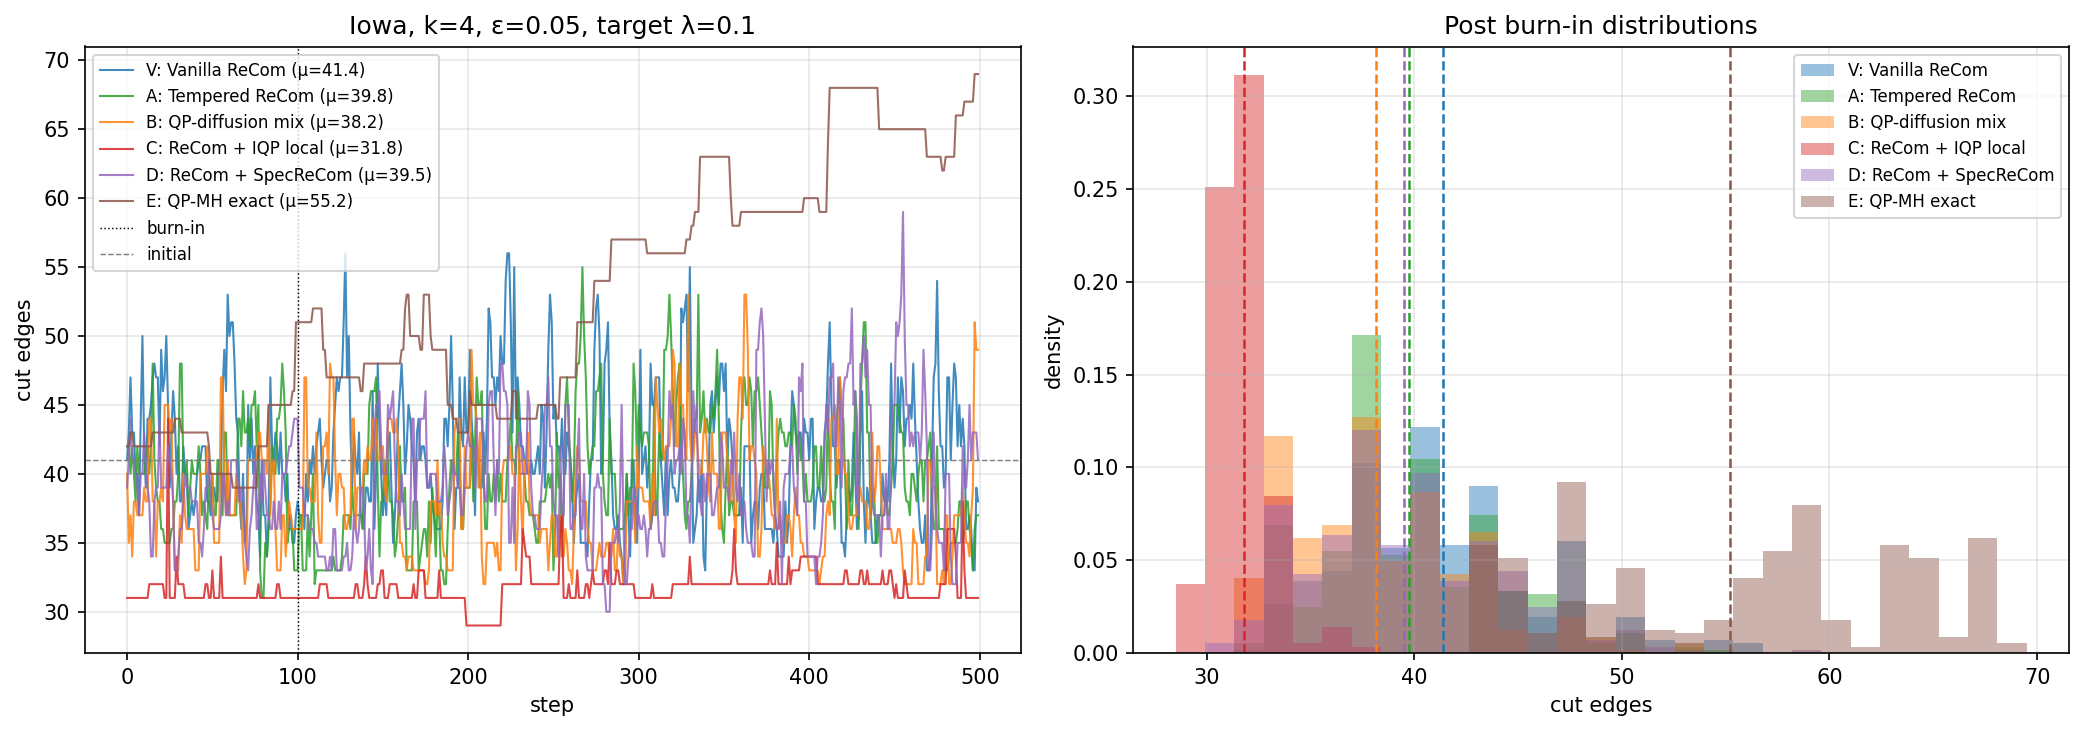
\includegraphics[width=0.92\textwidth]{fig/target_matched_iowa.png}
  \caption{Cut-edge trace and post-burn-in histogram for the six
    chains on Iowa. Chain C concentrates tightly at low cut counts;
    Chain E drifts upward toward the tempered target's own cut
    level.}
  \label{fig:iowa-trace}
\end{figure}

The wall-clock column completes the practitioner picture. Chain C's
compactness costs $\sim 47\times$ the per-step time of Vanilla ReCom at
$n_{\mathrm{iqp}} = 10$ (about 0.11\,s per step on Iowa), which is
acceptable for ensembles of thousands of plans but material at
precinct scale. Chain C's tight standard deviation (1.25 vs.\ 4.32
for A) is the signature of an optimizer concentrating on IQP local
minima rather than the spread of a sampler at equilibrium, consistent
with its matheuristic reading (\S\ref{sec:chain-c-honest}).

\paragraph{Optimizer baselines.}\label{sec:exp-optimizer-baselines}
Because Chain C is benchmarked as an optimizer, we compare it against
the classical optimizers a referee should demand. Simulated annealing
over ReCom proposals (the same Metropolis filter as Chain A with a
geometric cooling schedule, $\lambda$ from $0.05$ to $5$) and pure
hill climbing (accept only non-worsening moves) both cost the same as
Vanilla ReCom, about one second for 500 steps on Iowa. We also run
the same schedule stretched to $5\,000$ steps and a 25-restart
variant.

\begin{table}[htbp]
\centering
\small
\begin{tabular}{lrrrrr}
\toprule
Method & Best cuts & Ensemble mean & Distinct plans & Pairwise dist. & Wall \\
\midrule
SA (500 steps)           & 31 & 31    & 1 (frozen)  & ---  & 1.0\,s \\
Hill climbing (500)      & 31 & 31    & 1 (frozen)  & ---  & 0.9\,s \\
SA (5\,000 steps)        & 29 & 31    & 1 (frozen)  & ---  & 9.7\,s \\
SA, 25 restarts          & 29 & 31.00 & 23          & 25.1 & 26\,s \\
Vanilla ReCom + IQP      & 31 & 31.68 & moving      & ---  & 53\,s \\
Chain C                  & 29 & 32.34 & 135         & 23.5 & 57\,s \\
\bottomrule
\end{tabular}
\caption{Optimizer baselines on Iowa (seed 42,
  Gurobi 13). ``Ensemble mean'' is the mean cut count of the plans
  each method ends up producing (the frozen plateau for single-run
  SA and hill climbing, the set of 23 distinct final plans for
  restarted SA, the distinct post-burn-in plans for the chain
  methods). ``Distinct plans'' counts distinct plans produced (over
  400 post-burn steps for Chain C). ``Pairwise dist.''\ is the mean
  number of counties reassigned between two distinct plans under the
  best district relabeling. The single-run SA and hill-climbing rows
  were replicated across ten seeds. SA's best ranges over 30--32 and
  never reaches 29 in 500 steps (mean frozen plateau 31.8), and hill
  climbing lands at 31 on every
  seed.}\label{tab:optimizer-baselines}
\end{table}

We report this comparison as a main finding rather than bury it, and
it cuts both ways. The best plan quality found (29 cut edges) is
reached by three routes, namely the $5\,000$-step anneal (9.7\,s),
restarted annealing (26\,s), and Chain C (57\,s). For a
\emph{single} compact plan, the longer anneal is the clear winner at
about a sixth of Chain C's cost, so nobody should reach for an MIQP
to find one compact map. As \emph{ensemble} generators the two are
closer. At under half of Chain C's wall-clock, restarted annealing yields a
slightly better mean over its distinct plans (31.00 vs.\ 32.34) and
slightly higher diversity (25.1 vs.\ 23.5 counties reassigned between
plan pairs), while Chain C yields far more distinct near-optimal
plans per minute (about 141 vs.\ 53). Neither dominates. A
$2 \times 2$
decomposition sharpens where the compactness comes from. Adding IQP
refinement to Vanilla ReCom is worth about $10$ cuts on the mean
(41.39 to 31.68) and adding it to Tempered ReCom about $8$ (39.76 to
31.78), while the tempering filter alone is worth about $1.6$ cuts
and moves the post-refinement mean by under $0.2$. The optimizer does
the work; the outer filter barely moves the mean, though on this seed
only the tempered variant reached a 29-cut plan.

Two conclusions follow. On pure compactness optimization the classical
baseline matches the MIQP machinery at a fraction of the cost, and we
believe papers in the optimization-inside-ReCom line should report
it as standard practice. What the energy retains is anchoring, small
changes near a given plan, tested head to head in
\S\ref{sec:exp-leastchange}, together with kernel flexibility
(\S\ref{sec:exp-multikernel}) and, in Chain E, a provable stationary
distribution that no annealing schedule provides.

\subsection{North Carolina precinct validation}\label{sec:exp-nc}
We repeat the six-chain comparison on the North Carolina precinct dual
graph (\texttt{NC\_VTD}, $2\,692$ precincts, $k = 4$,
$\varepsilon = 0.05$, seed 42, 500 steps), roughly twenty-seven times
the vertex count of the Iowa instance. This is a single-seed scale
demonstration, so we report effect sizes without ESS-corrected test
statistics and read the directions, not the exact magnitudes.

\begin{table}[htbp]
\centering
\small
\begin{tabular}{lrrlr}
\toprule
Chain & Mean cuts & Std & $\Delta$ vs A (Cohen's $d$) & Wall-clock \\
\midrule
V: Vanilla ReCom    & 302.5 & 37.9 & ---                & 31\,s \\
A: Tempered ReCom   & 226.4 & 23.8 & ---                & 30\,s \\
B: QP-diffusion mix & 252.6 & 50.9 & $+11.5\%$ ($+0.66$) & 89\,s \\
\textbf{C: IQP local ($n_{\mathrm{iqp}} = 10$)}
                    & \textbf{145.7} & \textbf{3.9}
                    & \textbf{$-35.7\%$ ($-4.73$)} & 1950\,s \\
D: Spectral mix     & 253.7 & 49.8 & $+12.0\%$ ($+0.70$) & 131\,s \\
E: QP-MH exact      & 418.6$^{\dagger}$ & 25.1 & n/a (not converged) & 91\,s \\
\bottomrule
\end{tabular}
\caption{North Carolina precincts ($k = 4$, $\varepsilon = 0.05$,
  500 steps, burn-in 100, seed 42, per-step balance audit passed).
  Chain C reduces mean cut edges by $35.7\%$ versus Tempered ReCom,
  a larger relative gain than on Iowa, at a per-step cost of about
  $3.9$\,s. $^{\dagger}$Chain E is still climbing at 500 steps and its
  mean is a non-equilibrium lower bound, as on Iowa.}\label{tab:nc-headline}
\end{table}

Two things carry over from Iowa and one is new. The integer refinement
again dominates its chain family, and by a wider margin
($-35.7\%$, $d = -4.73$), consistent with our reading that
heterogeneous real-world graphs leave more room for local
optimization than the uniform grid. Chain C's distribution is again
sharply concentrated (std $3.9$ against $23.8$ for A). The new
observation is that on this larger graph the two mixture chains, B and
D, land \emph{above} Tempered ReCom rather than beside it ($+11.5\%$
and $+12.0\%$), because a single continuous QP solve or spectral cut
on a precinct-scale merged region is a coarse move that the
unconditional accept step does not filter, so at scale the cheap
regimes hurt. Only the exact integer solve (Chain C) and the exact
sampler (Chain E, by construction) behave well at precinct scale. The
cost is real. Chain C's $1950$\,s for 500 steps, about $3.9$\,s per
step, is acceptable for a targeted refinement pass but not for a long
ensemble run, which is the same speed-versus-power trade the Iowa
timings show, magnified by scale.

\subsection{Multi-kernel showcase on Iowa}\label{sec:exp-multikernel}

We run Chain B and Chain C on Iowa with three kernels and visualize
the resulting partitions. The three kernels are uniform
($k_{\mathrm{unif}}$), perimeter ($k_{\mathrm{perim}}$,
$w_{ij}$ = shared-boundary length from \texttt{shared\_perim}), and
density ($k_{\mathrm{dens}}$, $w_{ij} = |\partial v_i \cap \partial v_j| \cdot \exp(-(\rho_i - \rho_j)^2 / \sigma^2)$
with $\rho_v = \mathrm{TOTPOP}/\mathrm{area}$ normalized to unit
mean and $\sigma = 1$).

\begin{figure}[htbp]
  \centering
  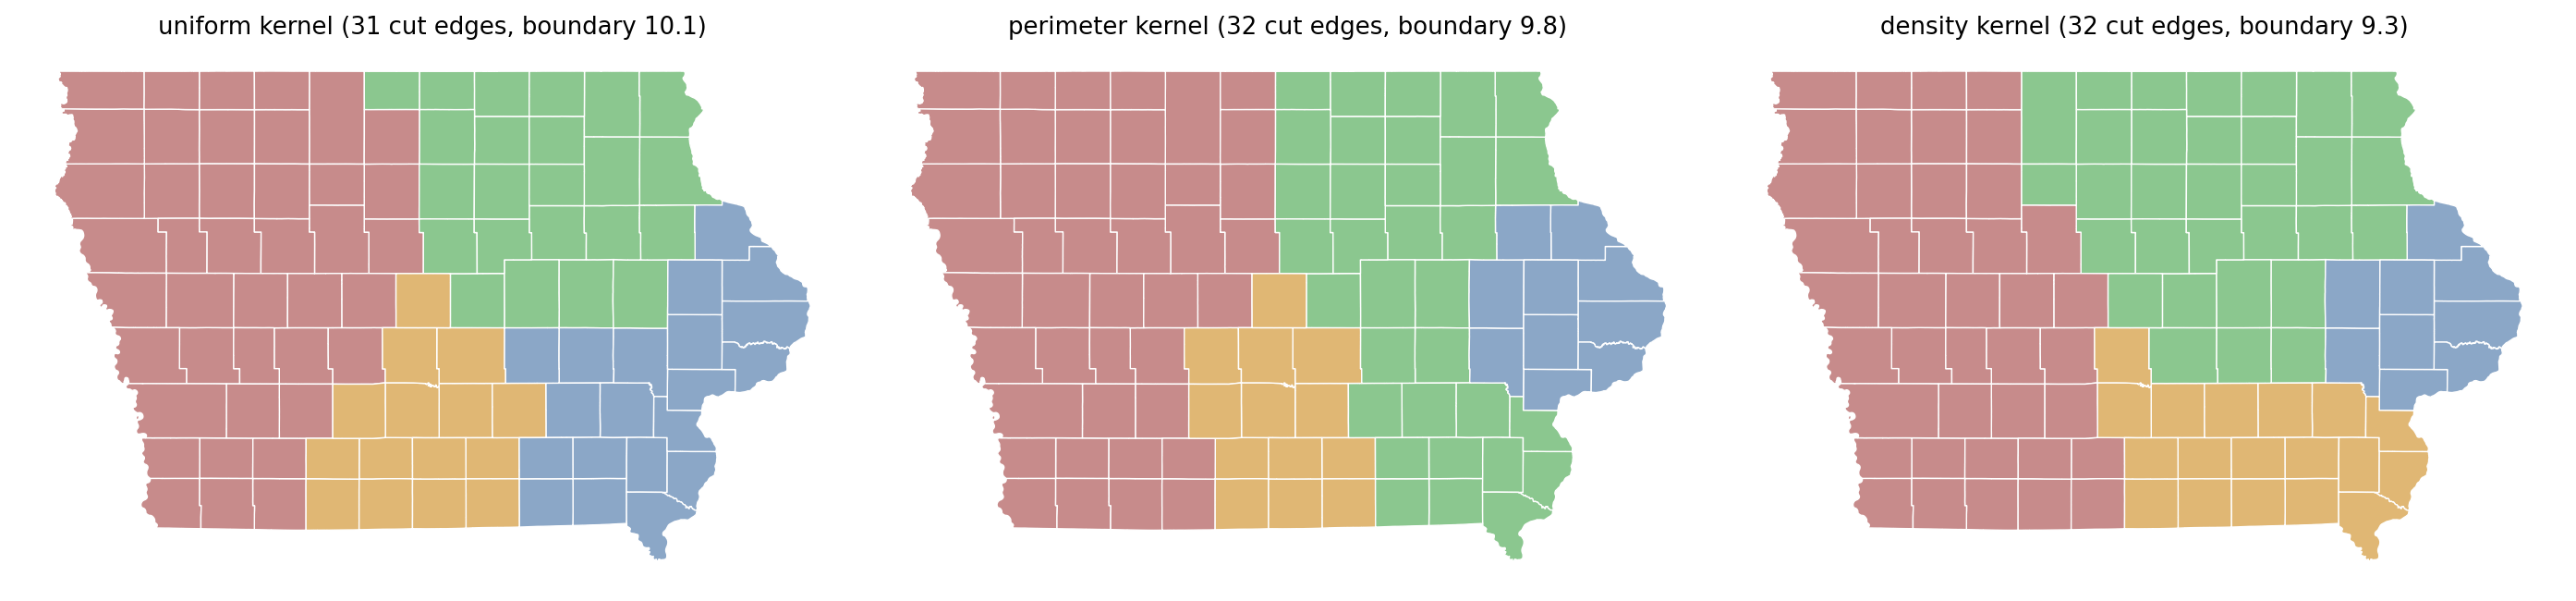
\includegraphics[width=\textwidth]{fig/multikernel_iowa.png}
  \caption{Final Chain C plans on Iowa under the three kernels
    (seed 42, 500 steps, identical constraints; only the Laplacian
    edge weights differ). Panel annotations give the unweighted cut
    count and the geographic boundary length (sum of shared-perimeter
    weights over cut edges). The plans differ in 19 to 25 of the 99
    counties under optimal district relabeling. The kernel directly
    encodes geographic signal at the proposal level.}
  \label{fig:multikernel-iowa}
\end{figure}

\begin{table}[htbp]
\centering
\small
\begin{tabular}{lrrrr}
\toprule
Kernel & B mean cuts & C mean cuts & C boundary (mean $\pm$ sd)
  & C $|\Delta\rho|$ ratio (mean $\pm$ sd) \\
\midrule
$k_{\mathrm{unif}}$  & 38.15 & 31.78 & $10.38 \pm 0.67$ & $1.78 \pm 0.36$ \\
$k_{\mathrm{perim}}$ & 39.00 & 33.39 & $\mathbf{9.89 \pm 0.42}$ & $1.82 \pm 0.39$ \\
$k_{\mathrm{dens}}$  & 38.09 & 36.84 & $11.31 \pm 1.16$ & $\mathbf{2.07 \pm 0.37}$ \\
\bottomrule
\end{tabular}
\caption{Three kernels on Iowa ($k = 4$, $\varepsilon = 0.05$,
  500 steps, burn-in 100, seed 42, corrected balance constraint,
  Gurobi 13). Mean cuts are post-burn-in averages of the unweighted
  cut count. The last two columns are averaged over every post-burn-in
  Chain C plan (not one snapshot), with the standard deviation across
  plans. ``C boundary'' is the geographic boundary length (sum of
  \texttt{shared\_perim} over cut edges, in the dual graph's units).
  ``$|\Delta\rho|$ ratio'' is the mean population-density gap across
  cut edges divided by the graph-wide mean gap, so $1.00$ means
  density-blind boundaries and larger values mean boundaries
  concentrated on urban--rural transitions. Each kernel is best on its
  own metric (bold): the perimeter kernel gives the shortest
  geographic boundary, the density kernel the highest density-gap
  ratio. Under non-uniform kernels the unweighted cut count is not the
  objective, so the cut columns must be read together with the
  kernel-specific columns.}\label{tab:multikernel-iowa}
\end{table}

\textbf{What each kernel does to the plan.} The three final Chain C
plans in Figure~\ref{fig:multikernel-iowa} disagree on 19 to 25 of 99
counties under the best district relabeling, and averaged over the
post-burn-in trajectory each kernel is best on the quantity it
encodes (Table~\ref{tab:multikernel-iowa}). The density kernel
accepts a longer border in exchange for aligning cuts with
population-density transitions; its four largest-gap cut edges are
the borders of Polk County (Des Moines), then Linn (Cedar Rapids) and
Johnson (Iowa City), the state's three urban cores, rather than edges
through uniformly rural blocks.

We stress the trajectory averages over single-plan snapshots on
purpose. A single final plan is a noisy draw, and its boundary and
gap numbers can point the wrong way. Figure~\ref{fig:multikernel-iowa}
itself illustrates this. The final density-kernel plan happens to land
a shorter boundary than the final perimeter plan, opposite to the
trajectory means. Only the post-burn-in means, with the
spreads in Table~\ref{tab:multikernel-iowa}, separate the kernel's
systematic effect from run-to-run noise.

\textbf{Reading the cut-count column.} Chain B is nearly
kernel-insensitive (38.1--39.0 mean cuts across all three),
consistent with its Iowa null result. The continuous relaxation plus
rounding does not transmit the kernel's signal into the final integer
plan the way the exact integer solve does.

\subsection{Least-change refinement from the enacted plan}\label{sec:exp-leastchange}

Remedial redistricting often asks for the smallest change that
improves a specific plan, for example when a commission must repair a
defect without redrawing the whole map. This is the setting the
fidelity term was built for, and we quantify it directly. The
reference plan is Iowa's enacted 2011 congressional map (47 cut
edges; district populations within $0.01\%$ of the ideal, so it is a
valid state of every chain in this paper). A method may reassign at
most $D$ of the 99 counties, counted under the best district
relabeling, and we record the best cut count it achieves within that
budget, over ten seeds.

Three methods start at the reference. The \emph{anchored IQP
refinement} is the paper's inner move alone ($\alpha = 10$, uniform
kernel, global balance window, no outer ReCom move), run for 50
passes. Because the fidelity weight $\beta$ is exactly the
least-change dial, the method's frontier is the envelope of (cuts,
distance) trajectories over $\beta \in \{0, 0.3, 1, 3, 10, 30\}$,
about 3\,s of total solve time per seed. \emph{Distance-capped
annealing over ReCom proposals} uses the geometric schedule of
\S\ref{sec:exp-optimizer-baselines} and rejects any proposal beyond
the budget ($2\,000$ proposals per budget, about 4\,s).
\emph{Distance-capped annealing over single-county boundary flips},
with contiguity and the global balance window enforced per flip, is
the fine-grained classical alternative ($2\,000$ proposals, under
1\,s).

\begin{table}[htbp]
\centering
\small
\begin{tabular}{rrrr}
\toprule
Budget $D$ & IQP anchored ($\beta$ envelope) & SA-ReCom capped & SA-flip capped \\
\midrule
3  & $42.40 \pm 1.36$ & $41.40 \pm 0.80$ & $\mathbf{40.60 \pm 0.66}$ \\
5  & $39.60 \pm 0.92$ & $38.80 \pm 0.75$ & $\mathbf{38.20 \pm 0.40}$ \\
10 & $\mathbf{32.00 \pm 0.00}$ & $32.10 \pm 0.30$ & $33.10 \pm 0.94$ \\
15 & $32.00 \pm 0.00$ & $\mathbf{31.70 \pm 0.46}$ & $32.10 \pm 0.30$ \\
20 & $32.00 \pm 0.00$ & $\mathbf{31.20 \pm 0.40}$ & $31.60 \pm 0.49$ \\
none & $31.80 \pm 0.40$ & $\mathbf{30.60 \pm 0.66}$ & $32.30 \pm 0.46$ \\
\bottomrule
\end{tabular}
\caption{Least-change refinement of the enacted Iowa plan (47 cut
  edges). Entries are the best cut count reachable while reassigning
  at most $D$ counties (best district relabeling), mean $\pm$ sd over
  ten seeds; bold marks the best method per budget. The last row
  removes the cap ($D = 99$).}\label{tab:least-change}
\end{table}

Move granularity explains the pattern. From the reference, an
accepted ReCom move reassigns a median of 26 counties (mean 25.0,
minimum 1 over 197 accepted moves), so the capped ReCom annealer
survives on the rare tree draws that happen to re-split almost
identically. An accepted IQP pass at $\beta = 1$ moves 2.5 counties
on average (median 2, maximum 5).

No method dominates the frontier, and we report all three regimes.
At tight budgets ($D \le 5$) capped flip annealing wins; one-county
moves explore the small-perturbation space that both the tree
re-split and the pair-optimal IQP step overshoot. At $D = 10$ the
anchored refinement ties the capped ReCom annealer ($32.00$ against
$32.10 \pm 0.30$, inside one standard deviation) and, unlike the
annealers, it is deterministic. From the enacted plan the $\beta = 1$ refinement
removes 15 of 47 cut edges while moving exactly 10 counties, reaching
the same plan on all ten seeds in about half a second of solve time,
with no cooling schedule or restart budget to tune. At loose budgets
($D \ge 15$) the task stops being least-change and capped ReCom
annealing pulls ahead, consistent with
\S\ref{sec:exp-optimizer-baselines}. The practical summary is that
for repairs moving roughly ten percent of units the anchored IQP
matches the best annealer and is the only reproducible method,
smaller repairs favor flip annealing, and larger redraws favor global
annealing. An exact benchmark for this setting exists in the
transfer-distance midpoint programs of Dobbs et
al.~\cite{dobbs2024facilitating}, and comparing against it is the
natural next step for this experiment. The IQP
frontier here came from sweeping $\beta$, which confirms the fidelity
term as a usable least-change dial rather than a fixed setting.

%════════════════════════════════════════════════════════════════════════════════
\section{Ablations and sensitivity}\label{sec:exp-ablations}
%════════════════════════════════════════════════════════════════════════════════



All tables in this appendix are from the corrected balance
constraint and Gurobi 13, on the same Chain C RNG stream as the
headline table.

\paragraph{Diversity controls (Jitter and Tabu).}\label{sec:exp-diversity}

\begin{table}[htbp]
\centering
\small
\begin{tabular}{lrrrr}
\toprule
Configuration & Mean cuts & Std & Distinct-plan rate & Wall-clock \\
\midrule
Baseline ($n_{\mathrm{iqp}} = 5$)               & 31.64 & 2.10 & 32.8\% & 31\,s \\
+ Jitter ($\mathcal{U}[1,2]$ on edge weights)   & 32.40 & 1.93 & \textbf{58.6\%} & 35\,s \\
+ Tabu (size 3)                                  & \textbf{30.16} & 1.60 & 14.6\% & 30\,s \\
\bottomrule
\end{tabular}
\caption{Diversity controls on Iowa ($n_{\mathrm{iqp}} = 5$,
  $\alpha = 10$, $\beta = 1$). ``Distinct-plan rate'' is the fraction
  of the 500 steps that produced a not-yet-seen plan. The two
  controls pull in opposite directions, as intended.}\label{tab:diversity-iowa}
\end{table}

Jitter varies which cut is taken on a given pair and buys exploration,
raising the distinct-plan rate from $33\%$ to $59\%$ at a cost of
under one cut. Tabu varies which pair is picked and buys depth,
forcing each step onto a boundary the chain has not just touched; it
deepens the optimization to the best mean in the paper while halving
the distinct-plan rate. A practitioner wanting a diverse ensemble
turns on Jitter; one wanting the sharpest compactness turns on Tabu.

\paragraph{Sensitivity to $n_{\mathrm{iqp}}$, $\alpha$, and $\beta$.}\label{sec:exp-sensitivity}

\begin{table}[htbp]
\centering
\small
\begin{tabular}{lrrr}
\toprule
Configuration & Mean cuts & $\Delta$ vs A & Wall-clock \\
\midrule
$n = 3, \alpha = 10, \beta = 1$  & 33.03 & $-16.9\%$ & 18\,s \\
$n = 5, \alpha = 10, \beta = 1$  & 31.64 & $-20.4\%$ & 31\,s \\
$n = 10, \alpha = 10, \beta = 1$ & 31.78 & $-20.1\%$ & 118\,s \\
$n = 3, \alpha = 50, \beta = 1$  & 32.70 & $-17.7\%$ & 24\,s \\
$n = 5, \alpha = 10, \beta = 0$  & 32.27 & $-18.8\%$ & 36\,s \\
$n = 10, \alpha = 50, \beta = 0$ & 31.19 & $-21.6\%$ & 196\,s \\
\bottomrule
\end{tabular}
\caption{Chain C parameter sensitivity on Iowa ($k = 4$,
  $\varepsilon = 0.05$, seed 42). $n_{\mathrm{iqp}}$ is the number of
  inner IQP passes per step. Wall-clock here wraps the whole run and
  was measured inside a 38-configuration sweep, whereas
  Table~\ref{tab:iowa-headline} sums per-step solve times on the same
  deterministic run, which is why the $n = 10$ row reads 118\,s here
  and 57\,s there. Compare rows within one table only.}\label{tab:sensitivity}
\end{table}

Table~\ref{tab:sensitivity} reports the uniform-kernel slice; the
full sweep over $n_{\mathrm{iqp}} \in \{3,5,10\}$,
$\alpha \in \{10,50\}$, $\beta \in \{0,1\}$ and all three kernels
(36 configurations) is released with the code as supplementary
material. Three readings. First, $n_{\mathrm{iqp}}$ has diminishing
returns.
Moving from $3$ to $5$ passes buys about three and a half percentage
points of cut reduction ($-17\%$ to $-20\%$), but moving from $5$ to
$10$ buys nothing more while multiplying the runtime by two to four
depending on the timing convention (see the caption), because after a
few passes the easy boundary improvements are exhausted and further
passes revisit already-refined pairs. Five passes is the practical
sweet spot. Second, $\alpha$ (the weight on the Laplacian smoothing
term) matters little once it is large enough to dominate. Moving from
$10$ to $50$ changes the result by half a cut or less, so we fix
$\alpha = 10$. Third, the
fidelity weight $\beta$ helps rather than hurts. At $n = 5$, keeping
$\beta = 1$ gives $-20.4\%$ against $-18.8\%$ with $\beta = 0$. The
anchor keeps each refinement near the current plan, which on
heterogeneous county populations lands better local optima than an
unanchored solve, and it is what the exactly reversible Chain E needs
to stay near-binary. We therefore keep $\beta = 1$ throughout.

%════════════════════════════════════════════════════════════════════════════════
\section{Discussion}\label{sec:discussion}
%════════════════════════════════════════════════════════════════════════════════

\subsection{Limitations}\label{sec:disc-limits}

\textbf{(L1) Chain B adds nothing significant on Iowa}
(\S\ref{sec:exp-compactness}); the relaxation appears too loose on
graphs with highly variable vertex populations.

\textbf{(L2) Integer QP is computationally expensive.} Chain C costs
$\sim 47\times$ Vanilla ReCom per step at $n_{\mathrm{iqp}} = 10$ on
Iowa. For precinct-scale graphs, time limits with warm starts (and
possibly coarsened merged-pair subproblems) will be necessary; the
NC experiment (\S\ref{sec:exp-nc}) is the pending scalability test.

\subsection{Future directions}\label{sec:disc-future}
\begin{enumerate}
  \item Benchmarking Chain C against exact cut-minimization optima on
    the public instances of Validi and
    Buchanan~\cite{validi2022political} and against the
    transfer-distance midpoint programs of Dobbs et
    al.~\cite{dobbs2024facilitating}.
  \item Replica exchange or parallel tempering between Chain C and
    sampling chains, in the spirit of multiscale parallel
    tempering~\cite{chuang2025multiscale}, to combine compactness with
    coverage.
  \item A kernel-faithful Cheeger sweep that scores candidates by
    weighted cut (\S\ref{sec:rounding}).
\end{enumerate}

%% TODO: conclusion.

\appendix
%════════════════════════════════════════════════════════════════════════════════
\section{Algorithm details and hyperparameters}\label{app:hyperparams}
%════════════════════════════════════════════════════════════════════════════════

\subsection{Common setup}\label{app:common}

\begin{itemize}
  \item Dual graph $G = (V, E)$ with vertex populations $p_v$ and
    edge attributes (\texttt{shared\_perim} for Iowa).
  \item $k$ districts, $\varepsilon$-population balance per
    Equation~\eqref{eq:pop-balance}, enforced as a two-sided bound around the
    global ideal on every move (Equation~\eqref{eq:balance-window})
    and audited per step. The bare GerryChain \texttt{recom} proposal
    is wrapped with an explicit whole-plan balance check
    (\texttt{recom\_valid}), since its internal cut search validates
    only one side of each split.
  \item Initial partition from
    \texttt{gerrychain.tree.recursive\_tree\_part}, redrawn until all
    $k$ districts satisfy the global tolerance
    (\texttt{balanced\_tree\_part}).
  \item Step count: $5 \times 5$: $N = 1\,000$, burn-in $B = 100$;
    Iowa: $N = 500$, $B = 100$; long-run validation
    (Paper~I, \S5.1): $2 \times 10^5$ (A) and
    $10^5$ (E) steps.
  \item Random seeds: base seed 42 with a distinct offset per chain
    (independent streams for Python \texttt{random} and
    \texttt{numpy}).
\end{itemize}

\subsection{Chain-specific parameters}\label{app:chains}

\begin{table}[htbp]
\centering
\small
\begin{tabular}{lll}
\toprule
Chain & Parameter & Value \\
\midrule
A & $\lambda$ (target temperature) & 0.10 \\
B & $p_R$ (ReCom mix probability) & 0.5 \\
B & $\alpha$ (Laplacian weight) & 10.0 \\
B & $\beta$ (fidelity weight) & 1.0 \\
B & Threshold scheme & Cheeger sweep, balance fallback \\
B & Laplacian normalization & False (unnormalized $L$) \\
C & $n_{\mathrm{iqp}}$ (IQP steps per outer iteration) & 10 \\
C & $\alpha$ & 10.0 \\
C & $\beta$ & 1.0 \\
C & MIQP time limit & 5.0 s \\
D & $p_R$ & 0.5 \\
D & Weight randomization & $\mathcal{U}[1, 2]$ per edge \\
D & Repair & False; balanced sweep in place of sign split \\
E & $\alpha$ & 1.0 \\
E & $\beta$ & 10.0 ($\tau = \alpha/\beta = 0.1$; Paper~I, Corollary~4.1 gives the resulting move size and Paper~I, \S4.7 places the mobility optimum near $\tau = 0.3$) \\
E & Rounding & single-shot Bernoulli($x^\star$) \\
E & $\lambda$ (MH target) & 0.10 \\
\bottomrule
\end{tabular}
\caption{Locked-in hyperparameters for the six
  chains.}\label{tab:hyperparams}
\end{table}

\subsection{Diversity controls}\label{app:diversity}

Weight jitter multiplies each edge weight by a draw from
$\mathcal{U}[1, 2]$ before solving (always on for D, as in Davies et
al.'s Algorithm~2; never used in Chain E, whose detailed-balance
argument needs a deterministic QP map). Tabu forbids the last $K = 3$
pairs chosen by the local kernel, cleared whenever ReCom moves.
Their effects are reported in Appendix~\ref{sec:exp-ablations}.

\subsection{Compute environment}\label{app:compute}

\begin{itemize}
  \item macOS (Darwin 23.6.0), Python 3.12.
  \item Gurobi 13.0.2 (academic license) for QP and MIQP, at its
    default thread count.
  \item NetworkX 3.x for graph operations.
  \item One Python process per run; no GPU. All experiments were run
    on a 2024 MacBook.
\end{itemize}

%════════════════════════════════════════════════════════════════════════════════
%════════════════════════════════════════════════════════════════════════════════
\subsection{Diversity controls}\label{app:diversity}

Weight jitter multiplies each edge weight by a draw from
$\mathcal{U}[1, 2]$ before solving (always on for D, as in Davies et
al.'s Algorithm~2; never used in Chain E, whose detailed-balance
argument needs a deterministic QP map). Tabu forbids the last $K = 3$
pairs chosen by the local kernel, cleared whenever ReCom moves.
Their effects are reported in Appendix~\ref{sec:exp-ablations}.


\bibliographystyle{plain}
\bibliography{ref}

\end{document}
